%%-*-latex-*-

%*******************************************************************************
\section{Evaluation}
%*******************************************************************************

One of the key concepts to be evaluated, with a focus on recursion, is
the hypothesis that novices would build abstract models more easily
when they experiment with tangible interfaces due to their didactic
virtues.

On this test, special interests has been putted on how lists work,
and, more specifically, how the their contents change through time
when exposed to recursive processes. The block\hyp{}world analogy is
expected to help understand the concept of list by physically
representing its main operations: \pop and \push and its LIFO (Last
Input First Output) behavior. Lists are then, the main data structure
in which recursion bases are built.

%*******************************************************************************
\subsection{Process}
%*******************************************************************************

The evaluation process is conducted with the help of 11 participants,
students from the faculties of Computer Science and Information
Technologies at Konkuk University. Their experience with functional
programming languages and concepts is very varied. Some of them had
never learn recursion or even wrote code in a functional language,
some others can be considered beginners and a final group are students
of the course of programming languages for postgraduates which is
focused on recursion by using \erlang.

The test consists in two parts. The first phase requires each
participant to solve the five exercises described in the section
\vref{sec:testcases}. The second phase is an exploratory survey that
participants are asked to complete.

The assistants are expected to complete the five exercises after a
brief explanation of how the interaction must be done. For simplicity
purposes the input of the problems does not contains more than 4 items
for each list, this means that they will be easy to solve. Only the
first exercise, \emph{Reverse}, is fully guided by a tutor who
explains the interactive process, provides additional information of
invalid actions and a course to follow. This means that \emph{Join},
\emph{Remove all}, \emph{Compress} and \emph{Insertion sort} are to be
solved entirely by the participant, the tutor is a supervisor during
these.

Finally, the survey is used to gather further information related to
the participant opinion of his experience and of the interface. An
introductory section has questions about previous knowledge of
recursion and functional programming. The main part of the
survey contains questions related to the participant experience with
the interface. Finally, the last part concludes with his personal
opinion of the interface and its benefits.

%*******************************************************************************
\subsection{Results}
%*******************************************************************************

The test is conducted in a total period of two weeks, each
participant's session lasts around 20 to 30 minutes and taking in
average 5 minutes per exercise. However, they do not have any time
constraint. After the experiment, several observations were made.

\begin{figure}
  \centering
  \subfigure{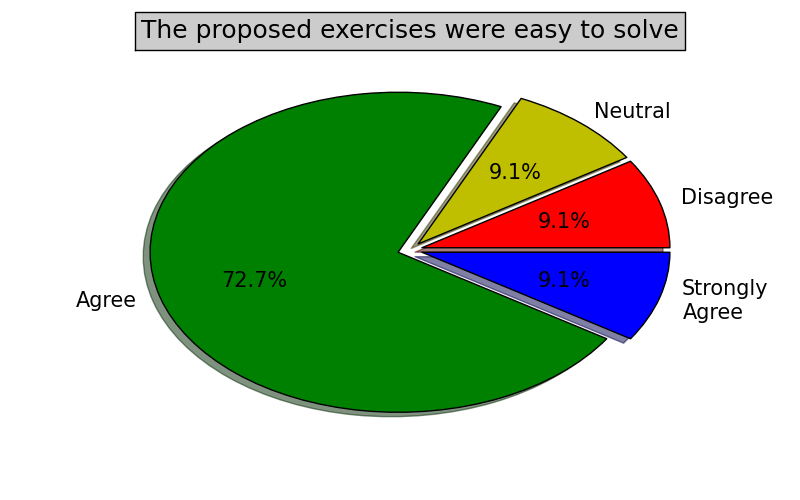
\includegraphics[width=0.47\textwidth]{img/survey/q4.png}\label{fig:survey:q4}}
  \subfigure{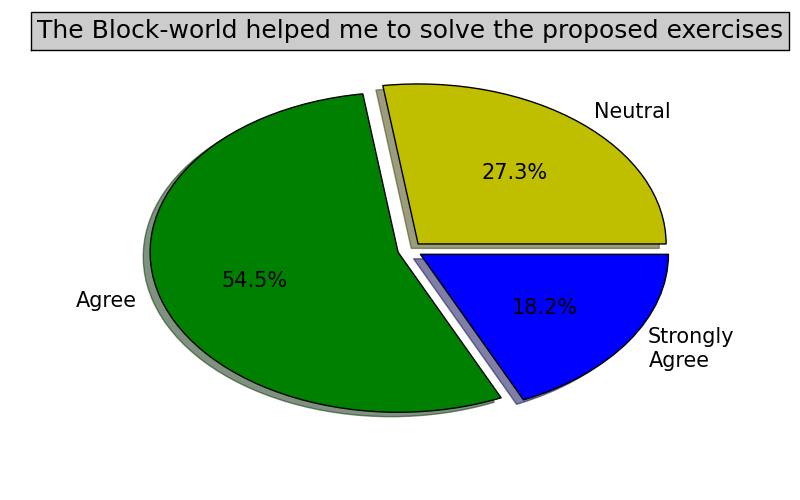
\includegraphics[width=0.47\textwidth]{img/survey/q5.png}\label{fig:survey:q5}}
  \subfigure{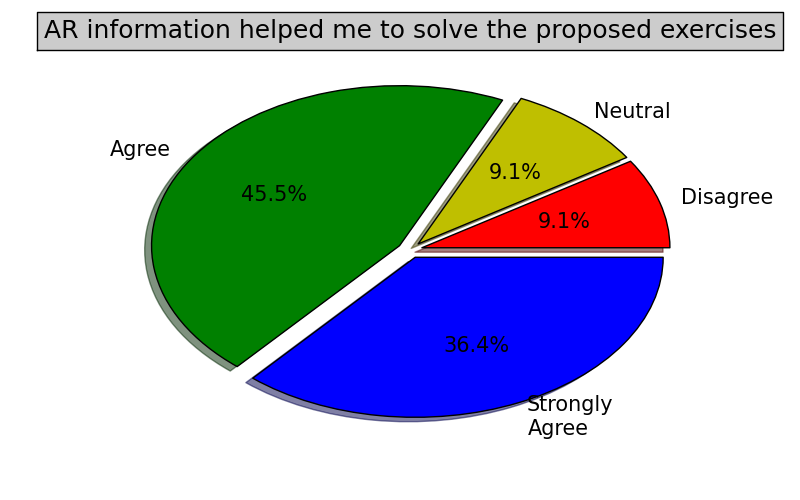
\includegraphics[width=0.47\textwidth]{img/survey/q6.png}\label{fig:survey:q6}}
  \subfigure{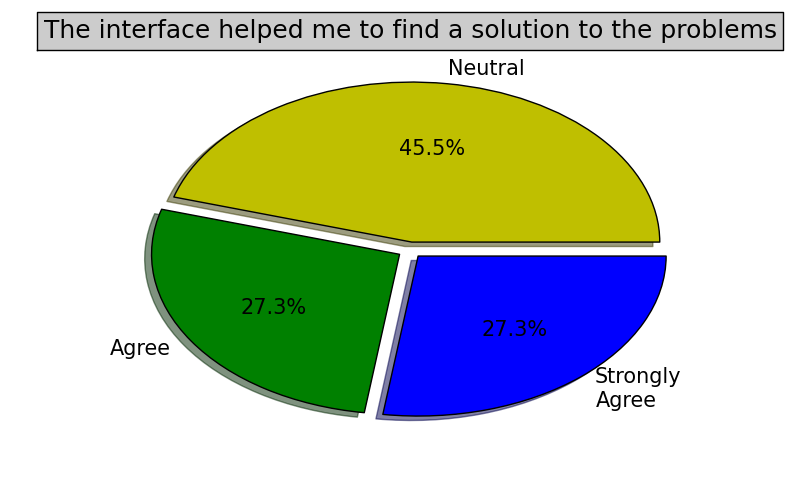
\includegraphics[width=0.47\textwidth]{img/survey/q7.png}\label{fig:survey:q7}}
  \caption{Survey questions, topic: interface exercises}
\end{figure}

One of the first observations is related to the progressive learning
process of the participants during the experiment. Most of them have
difficulties understanding the mechanics of the firsts two exercises
and serious mistakes are a very common event. However, they show an
important progress when solving the lasts problems, where nearly all
the mistakes are of minor importance. Further explanations were
required at the beginning of the session but as the participants
continued with it they progressively improve their problem solving
skills. For this reason, as seen in~\fig{fig:survey:q4}, the common
opinion is that the exercises are easy to solve.

The great majority of assistants agree that the combination of
Augmented Reality with the block\hyp{}world analogy provided a good
interface to solve the exercises. Their opinion is observed in the
questions in~\figs{fig:survey:q5}{fig:survey:q6}. Additionally,
more than half of the participants commented positively regarding to
how the interface helps to find out a solution to the exercises. This
question is found in~\fig{fig:survey:q7}. As a conclusion, the
application of these concepts was beneficial for the learning process.

\begin{figure}
  \centering
  \subfigure{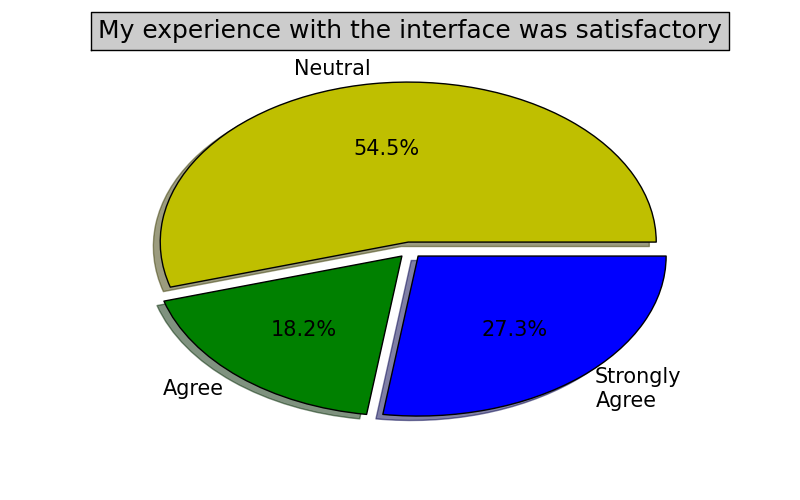
\includegraphics[width=0.47\textwidth]{img/survey/q9.png}\label{fig:survey:q9}}
  \subfigure{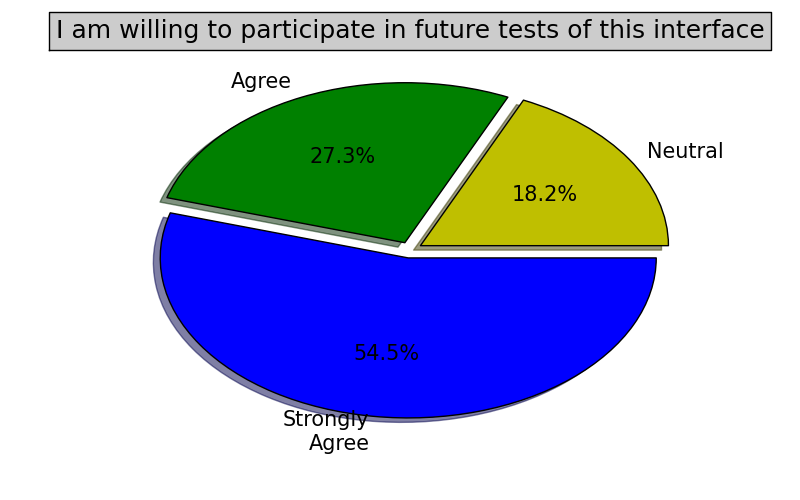
\includegraphics[width=0.47\textwidth]{img/survey/q11.png}\label{fig:survey:q11}}
  \subfigure{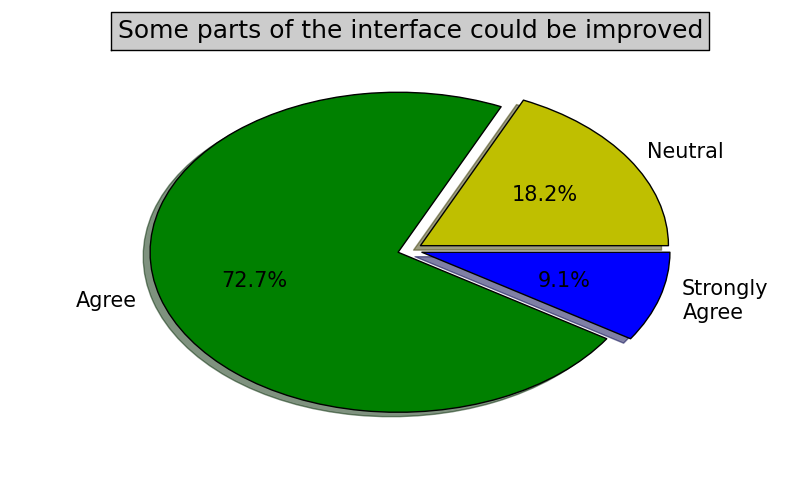
\includegraphics[width=0.47\textwidth]{img/survey/q10.png}\label{fig:survey:q10}}
  \caption{Survey questions, topic: general experience}
\end{figure}

Additionally, 45.5\% of the students have a good experience with the
interface and 81.8\% are willing to participate in future experiments,
this can be seen in more detail in~\fig{fig:survey:q9} and
in~\fig{fig:survey:q11}. Many of them complained about the fact that
every time a mistake is made the whole process should be restarted
from a valid initial state. This is one of the main critiques as
observed by the question in~\fig{fig:survey:q10} where 81.8\% of the
participants believe that several parts of the interface could be
improved. This interface's comportment underlies two intentions. The
first is to verify that the assistant can solve the each problem as a
whole and not just part of it; and the second is to use repetitions as
a form of punishing errors. Nevertheless, the opinions towards the
interface are positive.

\begin{figure}
  \centering
  \subfigure{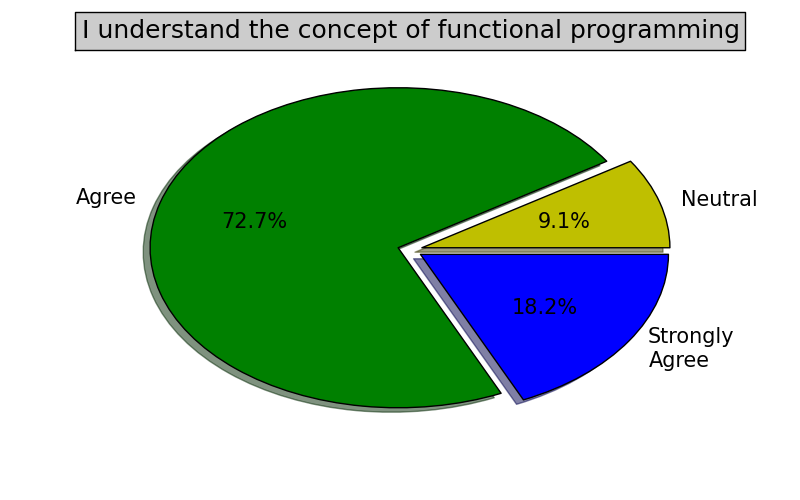
\includegraphics[width=0.47\textwidth]{img/survey/q1.png}\label{fig:survey:q1}}
  \subfigure{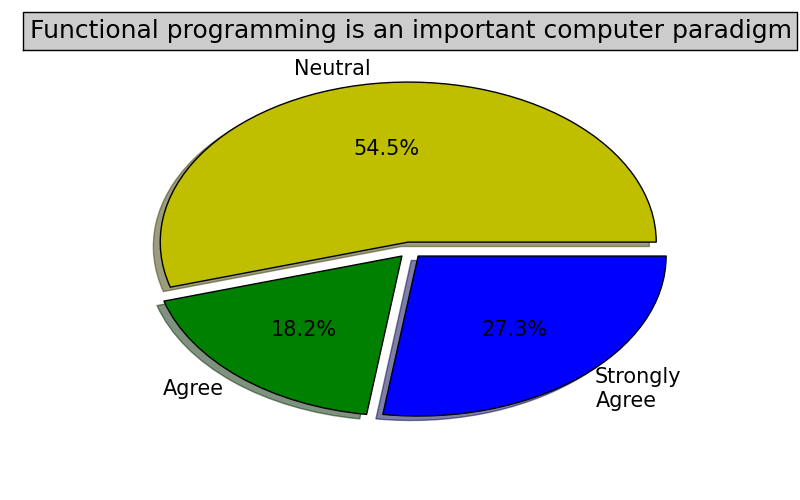
\includegraphics[width=0.47\textwidth]{img/survey/q3.png}\label{fig:survey:q3}}
  \subfigure{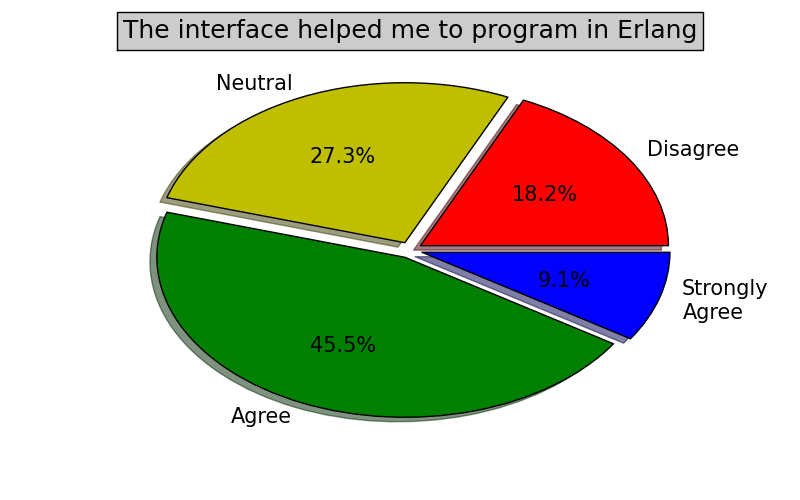
\includegraphics[width=0.47\textwidth]{img/survey/q8.png}\label{fig:survey:q8}}
  \subfigure{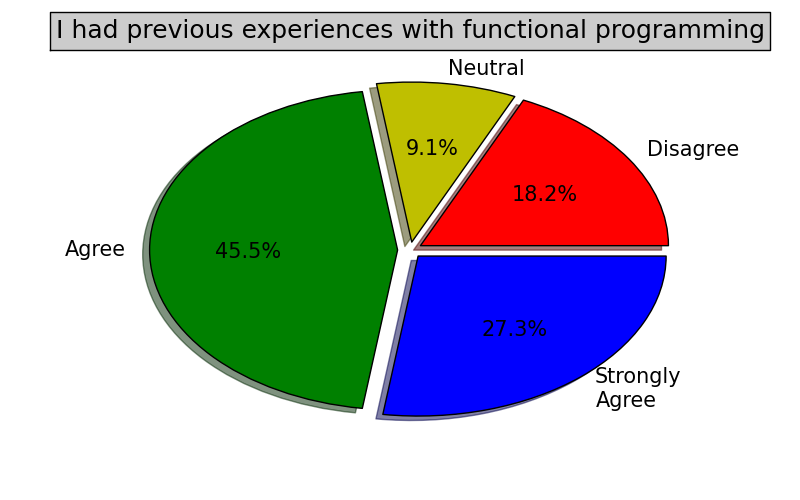
\includegraphics[width=0.47\textwidth]{img/survey/q2.png}\label{fig:survey:q2}}
  \caption{Survey questions, topic: functional programming}
\end{figure}

In the field of functional programming a curious event was observed.
Even though most of the participants have notions of understanding the
concept of functional programming, 54.5\% of them are neutral towards
considering it an important computer paradigm, this is shown
by~\fig{fig:survey:q1} and~\fig{fig:survey:q3}. This is a consequence
of colleges curriculum where \emph{object oriented} languages are
pervasive letting no space to different approaches. Therefore,
computer science students do not appreciate the benefits of using
functional programming languages.

Finally, only a small number of students, 18.2\%, commented that the
interface did not help them to learn \erlang, as shown
by~\fig{fig:survey:q8}. This remarkable development can occur by
several reasons. The first explanation relates the brevity of the
experiment where the proposed didactic phases are not followed.
However, longer sessions are expected to give a better understanding
of the \erlang-interface analogy and then transferring a
better training to the students. A second explanation is related to
participants' previous skills. As observed in~\fig{fig:survey:q2},
some students never have any contact with a functional programming
language, thus, making more difficult the process of learning. In
general, the feedback received in this point is very positive towards
the interface's purposes.
